\documentclass[10pt]{article}
\usepackage{amsmath}
\usepackage{graphicx}
\usepackage{geometry}
\usepackage{fancyhdr} % For header and footer
\usepackage{enumitem} % For customizing enumerate
\usepackage{tikz}
\usepackage{caption}
\usepackage{pgfplots}
\usetikzlibrary{3d,calc}
\geometry{letterpaper, margin=0.75in}
\renewcommand{\familydefault}{\sfdefault} % Use a sans-serif font

% Header and Footer
\pagestyle{fancy}
\fancyhf{}
\fancyhead[L]{EMCH 371 - Homework 2}
\fancyhead[R]{J. Vaught}
\fancyfoot[C]{\thepage}

% Title formatting
\title{\vspace{-2cm}\hrule\vspace{0.5cm}\\EMCH 371 - Homework 2\vspace{0.5cm}\hrule}
\author{\vspace{-1cm}J. Vaught}
\date{\vspace{-0.2cm}Due: Thursday, 9/26/2024}

\begin{document}
\maketitle

\vspace{-0.4cm}
\hrule
\vspace{0.5cm}

% Custom enumerate style
\begin{enumerate}[leftmargin=0.7cm, label=\textbf{\arabic*.}, itemsep=1em]

	\item Calculate the Atomic Packing Factor (APF) of 0.68 for the body-centered cubic (bcc) metal structure. (10pt)
	    \begin{itemize}[leftmargin=0.5cm]
        \item \textbf{Definition of APF:} The APF is the ratio of the volume of atoms in a unit cell to the total volume of the unit cell:
        \[
        \text{APF} = \frac{\text{Volume of atoms in the unit cell}}{\text{Total volume of the unit cell}}
        \]

        \item \textbf{Atoms in a bcc Unit Cell:} A bcc unit cell contains two atoms: one at the center and eight atoms at the corners (each contributing \( \frac{1}{8} \) atom per unit cell). The total number of atoms is:
        \[
        8 \times \frac{1}{8} + 1 = 2 \text{ atoms}
        \]

        \item \textbf{Volume of Atoms in the Unit Cell:} Let the atomic radius be \( r \). The volume of one atom is:
        \[
        \text{Volume of one atom} = \frac{4}{3} \pi r^3
        \]
        The total volume of atoms in the unit cell is:
        \[
        \text{Total volume of atoms} = 2 \times \frac{4}{3} \pi r^3 = \frac{8}{3} \pi r^3
        \]

        \item \textbf{Total Volume of the Unit Cell:} The body diagonal of the bcc unit cell is \( 4r \). The edge length \( a \) is related to the diagonal by:
        \[
        d = a\sqrt{3} \quad \text{so} \quad a = \frac{4r}{\sqrt{3}}
        \]
        The volume of the unit cell is:
        \[
        \text{Volume of unit cell} = a^3 = \left( \frac{4r}{\sqrt{3}} \right)^3 = \frac{64r^3}{3\sqrt{3}}
        \]

        \item \textbf{Calculation of APF:} Substituting the values into the APF formula:
        \[
        \text{APF} = \frac{\frac{8}{3} \pi r^3}{\frac{64r^3}{3\sqrt{3}}} = \frac{8 \pi}{64 \sqrt{3}} = \frac{\pi}{8 \sqrt{3}} \approx 0.68
        \]
        Thus, the APF for the bcc structure is approximately 0.68, indicating that 68\% of the unit cell's volume is occupied by atoms.
    \end{itemize}
    \begin{center}
    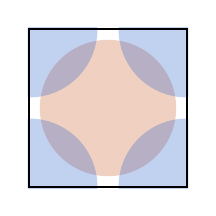
\begin{tikzpicture}
        % Define colors for atoms
        \definecolor{atomcorner}{rgb}{0.2, 0.4, 0.8} % Blueish color
        \definecolor{atomcenter}{rgb}{0.8, 0.4, 0.2} % Orangeish color
        
        % Define clipping path for the square
        \clip (-0.02,-0.02) rectangle (2.02,2.02);
        
        % Draw center atom
        \fill[atomcenter, opacity=0.3] (1,1) circle (0.866); % Center atom
        
        % Draw corner atoms
        \fill[atomcorner, opacity=0.3] (0,0) circle (0.866); % Bottom-left
        \fill[atomcorner, opacity=0.3] (2,0) circle (0.866); % Bottom-right
        \fill[atomcorner, opacity=0.3] (2,2) circle (0.866); % Top-right
        \fill[atomcorner, opacity=0.3] (0,2) circle (0.866); % Top-left
        
        % Draw unit square (side view of cube)
        \draw[black, thick] (0,0) -- (2,0) -- (2,2) -- (0,2) -- cycle; 
        \end{tikzpicture}
    \end{center}

    \newpage
	\item Calculate the APF of 0.74 for face-centered cubic (fcc) metals. (10pt)
	    \begin{itemize}[leftmargin=0.5cm]
        \item \textbf{Definition of APF:} The APF is the ratio of the volume of atoms in a unit cell to the total volume of the unit cell:
        \[
        \text{APF} = \frac{\text{Volume of atoms in the unit cell}}{\text{Total volume of the unit cell}}
        \]

        \item \textbf{Atoms in an fcc Unit Cell:} An fcc unit cell contains four atoms: eight corner atoms (each contributing \( \frac{1}{8} \) atom per unit cell) and six face-centered atoms (each contributing \( \frac{1}{2} \) atom per unit cell). The total number of atoms is:
        \[
        8 \times \frac{1}{8} + 6 \times \frac{1}{2} = 4 \text{ atoms}
        \]

        \item \textbf{Volume of Atoms in the Unit Cell:} Let the atomic radius be \( r \). The volume of one atom is:
        \[
        \text{Volume of one atom} = \frac{4}{3} \pi r^3
        \]
        The total volume of atoms in the unit cell is:
        \[
        \text{Total volume of atoms} = 4 \times \frac{4}{3} \pi r^3 = \frac{16}{3} \pi r^3
        \]

        \item \textbf{Total Volume of the Unit Cell:} In an fcc unit cell, the face diagonal is equal to four times the atomic radius, i.e., \( 4r \). For a cube, the face diagonal \( d_f \) is related to the edge length \( a \) by:
        \[
        d_f = a\sqrt{2} \quad \text{so} \quad a = \frac{4r}{\sqrt{2}} = 2\sqrt{2} r
        \]
        The volume of the unit cell is:
        \[
        \text{Volume of unit cell} = a^3 = \left( 2\sqrt{2} r \right)^3 = 16\sqrt{2} r^3
        \]

        \item \textbf{Calculation of APF:} Substituting the values into the APF formula:
        \[
        \text{APF} = \frac{\frac{16}{3} \pi r^3}{16\sqrt{2} r^3} = \frac{16 \pi}{48 \sqrt{2}} = \frac{\pi}{3 \sqrt{2}} \approx 0.74
        \]
        Thus, the APF for the fcc structure is approximately 0.74, indicating that 74\% of the unit cell's volume is occupied by atoms.
    \end{itemize}
    \begin{center}
        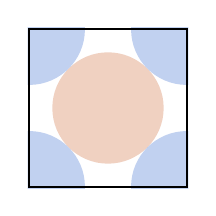
\begin{tikzpicture}
        
        % Define colors for atoms
        \definecolor{atomcorner}{rgb}{0.2, 0.4, 0.8} % Blueish color
        \definecolor{atomcenter}{rgb}{0.8, 0.4, 0.2} % Orangeish color
        
        % Define clipping path for the square
        \clip (-0.02,-0.02) rectangle (2.02,2.02);
        
        % Draw center atom
        \fill[atomcenter, opacity=0.3] (1,1) circle (0.707); % Center atom
        
        % Draw corner atoms
        \fill[atomcorner, opacity=0.3] (0,0) circle (0.707); % Bottom-left
        \fill[atomcorner, opacity=0.3] (2,0) circle (0.707); % Bottom-right
        \fill[atomcorner, opacity=0.3] (2,2) circle (0.707); % Top-right
        \fill[atomcorner, opacity=0.3] (0,2) circle (0.707); % Top-left
        
        % Draw unit square (side view of cube)
        \draw[black, thick] (0,0) -- (2,0) -- (2,2) -- (0,2) -- cycle; 
        \end{tikzpicture}
    \end{center}

    \newpage
	\item Assuming that \( r \) is the radius of \(\alpha\)-iron atom, the atomic packing factor of \(\alpha\)-iron, a body-centered cubic (BCC) metal, can be expressed by which of the following? (10pt)
    \begin{enumerate}[label=\textbf{\alph*.}, leftmargin=0.7cm, itemsep=0.5em]
        \item $\dfrac{\left( 4 \pi r^3 / 3 \right)}{\left( 4r / \sqrt{2} \right)^3}$
        
        \item $\dfrac{4 \left( 4 \pi r^3 / 3 \right)}{\left( 4r / \sqrt{3} \right)^3}$
        
        \item \fbox{$\dfrac{2 \left( 4 \pi r^3 / 3 \right)}{\left( 4r / \sqrt{3} \right)^3}$}
        
        \item $\left( \dfrac{4r / \sqrt{2}}{\left( 4 \pi r^3 / 3 \right)} \right)^3$
    \end{enumerate}
    
    \begin{itemize}[leftmargin=0.5cm]
        \item \textbf{Atoms in a BCC Unit Cell:} A BCC unit cell contains two atoms: one at the center and eight atoms at the corners, each contributing \( \frac{1}{8} \) atom per unit cell.
        \[
        8 \times \frac{1}{8} + 1 = 2 \text{ atoms}
        \]
        
        \item \textbf{Volume of Atoms in the Unit Cell:} The volume of one atom is given by:
        \[
        \text{Volume of one atom} = \frac{4}{3} \pi r^3
        \]
        For two atoms in the unit cell:
        \[
        \text{Total volume of atoms} = 2 \times \frac{4}{3} \pi r^3 = \frac{8}{3} \pi r^3
        \]
        
        \item \textbf{Total Volume of the Unit Cell:} The edge length \( a \) of the unit cell is related to the atomic radius \( r \) by:
        \[
        a = \frac{4r}{\sqrt{3}}
        \]
        Therefore, the volume of the unit cell is:
        \[
        \text{Volume of unit cell} = a^3 = \left( \frac{4r}{\sqrt{3}} \right)^3 = \frac{64r^3}{3\sqrt{3}}
        \]
        
        \item \textbf{Calculation of APF:} The APF is calculated as:
        \[
        \text{APF} = \frac{\frac{8}{3} \pi r^3}{\frac{64r^3}{3\sqrt{3}}} = \frac{8 \pi}{64 \sqrt{3}} = \frac{\pi}{8 \sqrt{3}}
        \]
        This corresponds to option \textbf{(c)}:
        \[
        \fbox{$\dfrac{2 \left( 4 \pi r^3 / 3 \right)}{\left( 4r / \sqrt{3} \right)^3}$}
        \]
    \end{itemize}

	\newpage
	\item Aluminum has a face-centered cubic unit cell.
    \begin{enumerate}[label=\textbf{\alph*.}, leftmargin=0.7cm, itemsep=0.5em]
        \item How many aluminum atoms are there in an aluminum unit cell? (10pt)
        
        \begin{itemize}[leftmargin=0.5cm]
            \item \textbf{Atoms in an FCC Unit Cell:} An FCC unit cell contains atoms at the corners and at the centers of each face of the cube. There are:
            \begin{itemize}
                \item 8 corner atoms, each contributing \(\frac{1}{8}\) atom per unit cell: 
                \[
                8 \times \frac{1}{8} = 1 \text{ atom}
                \]
                \item 6 face-centered atoms, each contributing \(\frac{1}{2}\) atom per unit cell:
                \[
                6 \times \frac{1}{2} = 3 \text{ atoms}
                \]
            \end{itemize}
            \item \textbf{Total number of atoms:}
            \[
            1 + 3 = 4 \text{ atoms}
            \]
            Thus, there are \textbf{4 aluminum atoms} in an aluminum unit cell.
        \end{itemize}

        \item \textbf{Calculate the density of aluminum (in g/cm\(^3\)).} (10pt)
        
        \begin{itemize}[leftmargin=0.5cm]
            \item \textbf{Atomic Mass of Aluminum:} The mass of one aluminum atom is given as:
            \[
            26.98 \text{ amu} = 26.98 \times 1.66 \times 10^{-24} \text{ g} = 4.48 \times 10^{-23} \text{ g}
            \]

            \item \textbf{Mass of Aluminum in a Unit Cell:} Since there are 4 atoms in the unit cell, the total mass is:
            \[
            4 \times 4.48 \times 10^{-23} \text{ g} = 1.79 \times 10^{-22} \text{ g}
            \]
            
            \item \textbf{Volume of the Unit Cell:} The edge length of the FCC unit cell for aluminum is approximately 0.405 nm.
            \[
            a = 0.405 \text{ nm} = 0.405 \times 10^{-7} \text{ cm} = 4.05 \times 10^{-8} \text{ cm}
            \]
            The volume of the unit cell is:
            \[
            V = a^3 = (4.05 \times 10^{-8} \text{ cm})^3 = 6.64 \times 10^{-23} \text{ cm}^3
            \]

            \item \textbf{Density of Aluminum:} The density is calculated as:
            \[
            \text{Density} = \frac{\text{Mass of unit cell}}{\text{Volume of unit cell}} = \frac{1.79 \times 10^{-22} \text{ g}}{6.64 \times 10^{-23} \text{ cm}^3} \approx 2.70 \text{ g/cm}^3
            \]
            Therefore, the density of aluminum is approximately \textbf{2.70 g/cm\(^3\)}.
        \end{itemize}
    \end{enumerate}

    
	\newpage
	\item Sketch in a cubic unit cell the [100] and [210] directions. (5pt each, total 10pt)

     \begin{center}
        \begin{tikzpicture}[scale=2]
            % Draw the unit cube
            \draw[thick] (0,0,0) -- (1,0,0) -- (1,1,0) -- (0,1,0) -- cycle;
            \draw[thick] (0,0,0) -- (0,0,1);
            \draw[thick] (0,0,1) -- (1,0,1) -- (1,1,1) -- (0,1,1) -- cycle;
            \draw[thick] (1,0,0) -- (1,0,1);
            \draw[thick] (1,1,0) -- (1,1,1);
            \draw[thick] (0,1,0) -- (0,1,1);

            % Axes
            \draw[->] (0,0,0) -- (1.2,0,0) node[anchor=north east]{$y$};
            \draw[->] (0,0,0) -- (0,1.2,0) node[anchor=north west]{$z$};
            \draw[->] (0,0,0) -- (0,0,1.3) node[anchor=south]{$x$};

            % Larger dots at the corners
            \foreach \x/\y/\z in {(0,0,0), (1,0,0), (1,1,0), (0,1,0), (0,0,1), (1,0,1), (1,1,1), (0,1,1)} {
                \node[circle,fill=black,inner sep=1.2pt] at (\x,\y,\z) {};
            }

            % [100] direction arrow
            \draw[line width=1mm, ->, purple] (0,0,0) -- (0,0,1);
        \end{tikzpicture}
        \captionsetup{type=figure}
        \captionof{figure}{[100] Direction in a Cubic Unit Cell}
       	     \begin{tikzpicture}[scale=2]
	      	% Draw the unit cube
	      	\draw[thick] (0,0,0) -- (1,0,0) -- (1,1,0) -- (0,1,0) -- cycle;
	      	\draw[thick] (0,0,0) -- (0,0,1);
	      	\draw[thick] (0,0,1) -- (1,0,1) -- (1,1,1) -- (0,1,1) -- cycle;
	      	\draw[thick] (1,0,0) -- (1,0,1);
	      	\draw[thick] (1,1,0) -- (1,1,1);
	      	\draw[thick] (0,1,0) -- (0,1,1);
	      	
	      	% Axes
	      	\draw[->] (0,0,0) -- (1.2,0,0) node[anchor=north east]{$y$};
	      	\draw[->] (0,0,0) -- (0,1.2,0) node[anchor=north west]{$z$};
	      	\draw[->] (0,0,0) -- (0,0,1.3) node[anchor=south]{$x$};
	      	
	      	% Larger dots at the corners
	      	\foreach \x/\y/\z in {(0,0,0), (1,0,0), (1,1,0), (0,1,0), (0,0,1), (1,0,1), (1,1,1), (0,1,1)} {
	      		\node[circle,fill=black,inner sep=1.2pt] at (\x,\y,\z) {};
	      	}
                % Dashed purple arrow from (0,0,0) to (0,1,1) with custom thickness
                \draw[line width=1mm, ->, blue] (0,0,0) -- (1,0,2);
	      \end{tikzpicture}
       \captionsetup{type=figure}
        \captionof{figure}{[210] Direction in a Cubic Unit Cell}
       \end{center}
	
	\item Iron typically has a body-centered cubic (BCC) structure at room temperature. Given that the iron atomic radius is 0.124 nm, determine in the iron unit cell:
    \begin{enumerate}[label=\textbf{\alph*.}, leftmargin=0.7cm, itemsep=0.5em]
        \item How many iron atoms per nm are there in the [111] direction? (10pt)
        \begin{itemize}[leftmargin=0.5cm]
            \item \textbf{Length of [111] direction:} The [111] direction corresponds to the body diagonal of the cubic unit cell. The length of the body diagonal is given by:
            \[
            d_{111} = \sqrt{3}a = 4r = 4 \times 0.124 \text{ nm} = 0.496 \text{ nm}
            \]

            \item \textbf{Number of atoms along [111] direction:} 
            The [111] direction passes through:
            \begin{itemize}
                \item 1 corner atom at the origin: \(\frac{1}{2}\) atom
                \item 1 atom at the center: 1 atom
                \item 1 corner atom at the other end: \(\frac{1}{2}\) atom
            \end{itemize}
            Thus, the total number of atoms is:
            \[
            \frac{1}{2} + 1 + \frac{1}{2} = 2 \text{ atoms}
            \]
            \[
            \text{Atoms per nm} = \frac{2 \text{ atoms}}{0.496 \text{ nm}} \approx 4.03 \text{ atoms/nm}
            \]
        \end{itemize}

        \item How many iron atoms per nm are there in the [110] direction? (10pt)
        \begin{itemize}[leftmargin=0.5cm]
            \item \textbf{Length of [110] direction:} The [110] direction corresponds to the face diagonal of the cubic unit cell. The length of the face diagonal is given by:
            \[
            d_{110} = \sqrt{2}a = \sqrt{2} \times \frac{4r}{\sqrt{3}} = \sqrt{2} \times 0.286 \text{ nm} = 0.405 \text{ nm}
            \]

            \item \textbf{Number of atoms along [110] direction:} 
            The [110] direction passes through:
            \begin{itemize}
                \item 1 corner atom at the origin: \(\frac{1}{2}\) atom
                \item 1 corner atom at the end: \(\frac{1}{2}\) atom
            \end{itemize}
            Thus, the total number of atoms is:
            \[
            \frac{1}{2} + \frac{1}{2} = 0.5 \text{ atoms}
            \]
            \[
            \text{Atoms per nm} = \frac{1.0 \text{ atoms}}{0.405 \text{ nm}} \approx 2.47 \text{ atoms/nm}
            \]
        \end{itemize}
    \end{enumerate}
	
    \item In a cubic lattice shown in Figures (a-b):
    \begin{enumerate}[label=\textbf{\alph*.}, leftmargin=0.7cm, itemsep=0.5em]
        \item Label the direction in Figure (a) (5pt) \\
              \textbf{Answer:} The direction from (0,0,0) to (1,0,1) is labeled as \textbf{[101] direction}.
        
        \item Label the shaded plane in Figure (b) (5pt) \\
              \textbf{Answer:} The plane passing through (1,0,0), (0,1,0), and (0,0,1) is labeled as \textbf{(111) plane}.
    \end{enumerate}

    \vspace{0.5cm}
    \begin{center}
	     \begin{tikzpicture}[scale=2]
	      	% Draw the unit cube
	      	\draw[thick] (0,0,0) -- (1,0,0) -- (1,1,0) -- (0,1,0) -- cycle;
	      	\draw[thick] (0,0,0) -- (0,0,1);
	      	\draw[thick] (0,0,1) -- (1,0,1) -- (1,1,1) -- (0,1,1) -- cycle;
	      	\draw[thick] (1,0,0) -- (1,0,1);
	      	\draw[thick] (1,1,0) -- (1,1,1);
	      	\draw[thick] (0,1,0) -- (0,1,1);
	      	
	      	% Axes
	      	\draw[->] (0,0,0) -- (1.5,0,0) node[anchor=north east]{$y$};
	      	\draw[->] (0,0,0) -- (0,1.5,0) node[anchor=north west]{$z$};
	      	\draw[->] (0,0,0) -- (0,0,1.5) node[anchor=south]{$x$};
	      	    
	      	% Dashed arrow from (0,0,0) to (0,1,1)
	      	\draw[thick, dashed, ->] (0,0,0) -- (0,2,2);
	      	
	      	% Larger dots at the corners
	      	\foreach \x/\y/\z in {(0,0,0), (1,0,0), (1,1,0), (0,1,0), (0,0,1), (1,0,1), (1,1,1), (0,1,1)} {
	      		\node[circle,fill=black,inner sep=1.2pt] at (\x,\y,\z) {};
	      	}
	      \end{tikzpicture}
       \begin{tikzpicture}[scale=2]
	      	% Draw the unit cube
	      	\draw[thick] (0,0,0) -- (1,0,0) -- (1,1,0) -- (0,1,0) -- cycle;
	      	\draw[thick] (0,0,0) -- (0,0,1);
	      	    
	      	% Shaded triangle
	      	\fill[red,opacity=0.5] (0,0,1) -- (1,0,0) -- (0,1,0) -- cycle;
	      	    
	      	\draw[thick] (0,0,1) -- (1,0,1) -- (1,1,1) -- (0,1,1) -- cycle;
	      	\draw[thick] (1,0,0) -- (1,0,1);
	      	\draw[thick] (1,1,0) -- (1,1,1);
	      	\draw[thick] (0,1,0) -- (0,1,1);
	      	
	      	% Axes
	      	\draw[->] (0,0,0) -- (1.5,0,0) node[anchor=north east]{$y$};
	      	\draw[->] (0,0,0) -- (0,1.5,0) node[anchor=north west]{$z$};
	      	\draw[->] (0,0,0) -- (0,0,1.5) node[anchor=south]{$x$};
	      	
	      	% Larger dots at the corners
	      	\foreach \x/\y/\z in {(0,0,0), (1,0,0), (1,1,0), (0,1,0), (0,0,1), (1,0,1), (1,1,1), (0,1,1)} {
	      		\node[circle,fill=black,inner sep=1.2pt] at (\x,\y,\z) {};
	      	}
	      \end{tikzpicture}
    \end{center}

    \item Clearly draw the [210] direction and the (011) plane in a cubic unit cell. (5pt each, total 10pt)
    
    \begin{center}    
	      \begin{tikzpicture}[scale=2]
	      	% Draw the unit cube
	      	\draw[thick] (0,0,0) -- (1,0,0) -- (1,1,0) -- (0,1,0) -- cycle;
	      	\draw[thick] (0,0,0) -- (0,0,1);
	      	\draw[thick] (0,0,1) -- (1,0,1) -- (1,1,1) -- (0,1,1) -- cycle;
	      	\draw[thick] (1,0,0) -- (1,0,1);
	      	\draw[thick] (1,1,0) -- (1,1,1);
	      	\draw[thick] (0,1,0) -- (0,1,1);
	      	
	      	% Axes
	      	\draw[->] (0,0,0) -- (2.2,0,0) node[anchor=north east]{$y$};
	      	\draw[->] (0,0,0) -- (0,2.2,0) node[anchor=north west]{$z$};
	      	\draw[->] (0,0,0) -- (0,0,2.3) node[anchor=south]{$x$};
	      	
	      	% Larger dots at the corners
	      	\foreach \x/\y/\z in {(0,0,0), (1,0,0), (1,1,0), (0,1,0), (0,0,1), (1,0,1), (1,1,1), (0,1,1)} {
	      		\node[circle,fill=black,inner sep=1.2pt] at (\x,\y,\z) {};
	      	}
	      	\foreach \x/\y/\z in {(2,0,0), (0,2,0), (0,0,2))} {
	      		\node[circle,fill=black,inner sep=0.8pt] at (\x,\y,\z) {};
	      	}
                        % Dashed purple arrow from (0,0,0) to (0,1,1) with custom thickness
                \draw[line width=0.5mm, dashed, ->, black] (0,0,0) -- (1,0,2);
	      \end{tikzpicture}
	      \begin{tikzpicture}[scale=2]
 % Draw the unit cube
    \draw[thick] (0,0,0) -- (1,0,0) -- (1,1,0) -- (0,1,0) -- cycle; % Bottom face
    \draw[thick] (0,0,0) -- (0,0,1); % Vertical edge back-left
    \draw[thick] (0,0,1) -- (1,0,1) -- (1,1,1) -- (0,1,1) -- cycle; % Top face
    \draw[thick] (1,0,0) -- (1,0,1); % Vertical edge front-right
    \draw[thick] (1,1,0) -- (1,1,1); % Vertical edge back-right
    \draw[thick] (0,1,0) -- (0,1,1); % Vertical edge front-left
    
    % Axes
    \draw[->] (0,0,0) -- (1.5,0,0) node[anchor=north east]{$y$};
    \draw[->] (0,0,0) -- (0,1.5,0) node[anchor=north west]{$z$};
    \draw[->] (0,0,0) -- (0,0,1.5) node[anchor=south]{$x$};
    
    % Larger dots at the corners
    \foreach \x/\y/\z in {(0,0,0), (1,0,0), (1,1,0), (0,1,0), (0,0,1), (1,0,1), (1,1,1), (0,1,1)} {
        \node[circle,fill=black,inner sep=1.2pt] at (\x,\y,\z) {};
    }
    
    % Shading the (110) plane
    \fill[blue, opacity=0.3] (1,0,0) -- (0,1,0) -- (0,1,1) -- (1,0,1) -- cycle;
	      \end{tikzpicture}
    \end{center}
    \newpage
	\item The lattice constant for a unit cell of fcc nickel is 0.325 nm.
	      \begin{enumerate}[label=\textbf{\alph*.}, leftmargin=0.7cm, itemsep=0.5em]
	      	\item Draw the (110) plane within a unit cell and show the atom center in the unit cell. (10pt)
	      	\item How many atoms are there per nm$^2$ on the (110) plane? Calculate the planar density of the (110) plane. (10pt)
	      \end{enumerate}

       \begin{center}
       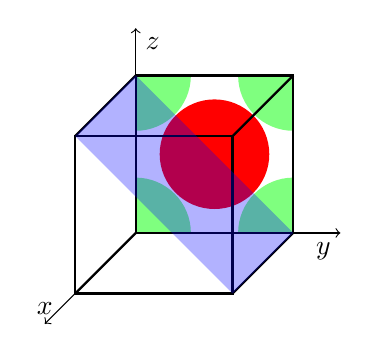
\begin{tikzpicture}[scale=2]
    \fill[green, opacity=0.5,] (0,0,0) -- (0.35,0,0) arc[start angle=0, end angle=90, radius=10pt] -- cycle;
    \fill[green, opacity=0.5,] (1,0,0) -- (1-0.35,0,0) arc[start angle=180, end angle=90, radius=10pt] -- cycle;
    \fill[green, opacity=0.5,] (1,1,0) -- (1-0.35,1,0) arc[start angle=180, end angle=270, radius=10pt] -- cycle;  
    \fill[green, opacity=0.5,] (0,1,0) -- (0.35,1,0) arc[start angle=360, end angle=270, radius=10pt] -- cycle;
    \node[circle, fill=red, inner sep=14pt] at (0.5,0.5,0) {}; % Atom at (0.5,0.5,0)

    \draw[thick] (0,0,0) -- (1,0,0) -- (1,1,0) -- (0,1,0) -- cycle; % Bottom face
    \draw[thick] (0,0,0) -- (0,0,1); % Vertical edge back-left
    \draw[thick] (0,0,1) -- (1,0,1) -- (1,1,1) -- (0,1,1) -- cycle; % Top face
    \draw[thick] (1,0,0) -- (1,0,1); % Vertical edge front-right
    \draw[thick] (1,1,0) -- (1,1,1); % Vertical edge back-right
    \draw[thick] (0,1,0) -- (0,1,1); % Vertical edge front-left
    
    % Label the axes
    \draw[->] (0,0,0) -- (1.3,0,0) node[anchor=north east]{$y$};
    \draw[->] (0,0,0) -- (0,1.3,0) node[anchor=north west]{$z$};
    \draw[->] (0,0,0) -- (0,0,1.5) node[anchor=south]{$x$};
    
    % Shading the (110) plane
     \fill[blue, opacity=0.3] (1,0,0) -- (0,1,0) -- (0,1,1) -- (1,0,1) -- cycle;
\end{tikzpicture}
\end{center}
    \begin{itemize}[leftmargin=0.5cm]
        \item \textbf{Atoms in the (110) Plane:} The (110) plane in FCC contains:
        \begin{itemize}[leftmargin=0.3cm]
            \item 4 corner atoms, each contributing \( \frac{1}{4} \) atom \( \Rightarrow 1 \text{ atom} \)
            \item 2 face-centered atoms \( \Rightarrow 2 \text{ atoms} \)
        \end{itemize}
        Total: \( 3 \) atoms in the (110) plane.

        \item \textbf{Area of the (110) Plane:}
        \[
        \text{Area} = a \times \sqrt{2}a = (0.325 \, \text{nm}) \times \sqrt{2} (0.325 \, \text{nm}) \approx 0.1495 \, \text{nm}^2
        \]

        \item \textbf{Planar Density:}
        \[
        \text{Planar Density} = \frac{\text{Number of atoms}}{\text{Area}} = \frac{3}{0.1495 \, \text{nm}^2} \approx 20.07 \, \text{atoms/nm}^2
        \]
    \end{itemize}

\end{enumerate}

\end{document}
